\chapter{Assessment} \label{chap:assessment}

The assessment was incremental. First, the aerodynamic properties were tested on a manual flight, qualitativaly, regarding properties such as stall angle, stall speed, and equilibrium point in flight. Following this, the hover capabilities were tested, such as altitude and atitude control. With the basic flight capabilities proven, a few autonomous, test flights were performed, without VTOL. Finally, it's VTOL capabilities were benchmarked. These tests are better described, as well as their results, in the following sections.


\section{Tethered Attitude Control Test}

To test the attitude control and stabilization, the prototype was hang by a rope, so it's range of movement was restricted, and it was safer to test indoors.
%
The first tests were qualitative. The wing was armed on the QStabilize mode, where the gyroscope and accelerometer are used to try to maintain the aircraft leveled in VTOL mode (propellers spinning parallel to ground).
%
The expected result was that the elevons should move trying to stop the movement, even without propellers on the motors (again, for safety reasons).
%
The aircraft successfully reacted to disturbances on it's attitude by moving the control surfaces appropriately.


\section{Un-tethered Attitude Control Test} 

For this test, the wing was taken to an open field on the university.
%
For the take-off, it had to be oriented so the wind blew parallel to it's surface, so that the wind didn't flip it over.
%
Take-off cant be too slow, as the winglets adhere to the the ground and can cause the aircraft to tip over.
%
once in the air, the controls and stabilization were good, but once the wind it the aircraft, it turned it perpendicular to the direction of the wind, and the control authority was not enough for both stabilizing flight and turning the yaw axis.
%
While this problem limits the yaw controllability in VTOL mode, the position control is not necessarily affected, as the aircraft can still move in a mixed attitude between VTOL and fixed wing, inclined against the wind and maintaining position.
%

This could possibly be fixed by increasing the winglets area, however this also increases the area the wind hits, and needs more testing to verify.
%

The flight path can be seen on Figure \ref{fig:flight1-3d}, and an in-fligt photo on Figure \ref{fig:flight1-photo}.
	
\begin{figure}[H]
\centering
  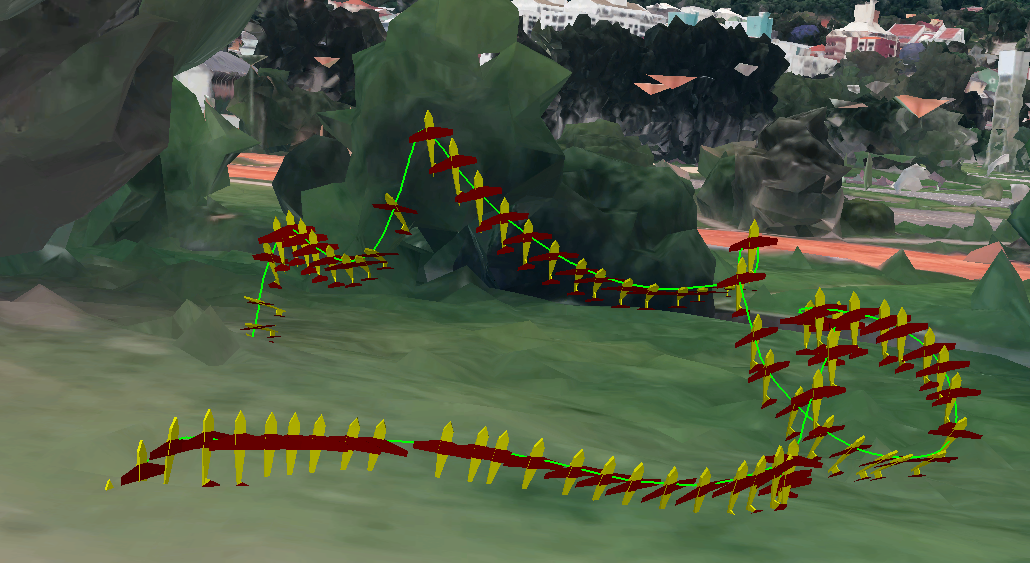
\includegraphics[width=0.7\linewidth]{figs/flight1-3d.png}
  \caption{Visualization of first test flight.}
  \label{fig:flight1-3d}
\end{figure}
	
	\begin{figure}[H]
\centering
  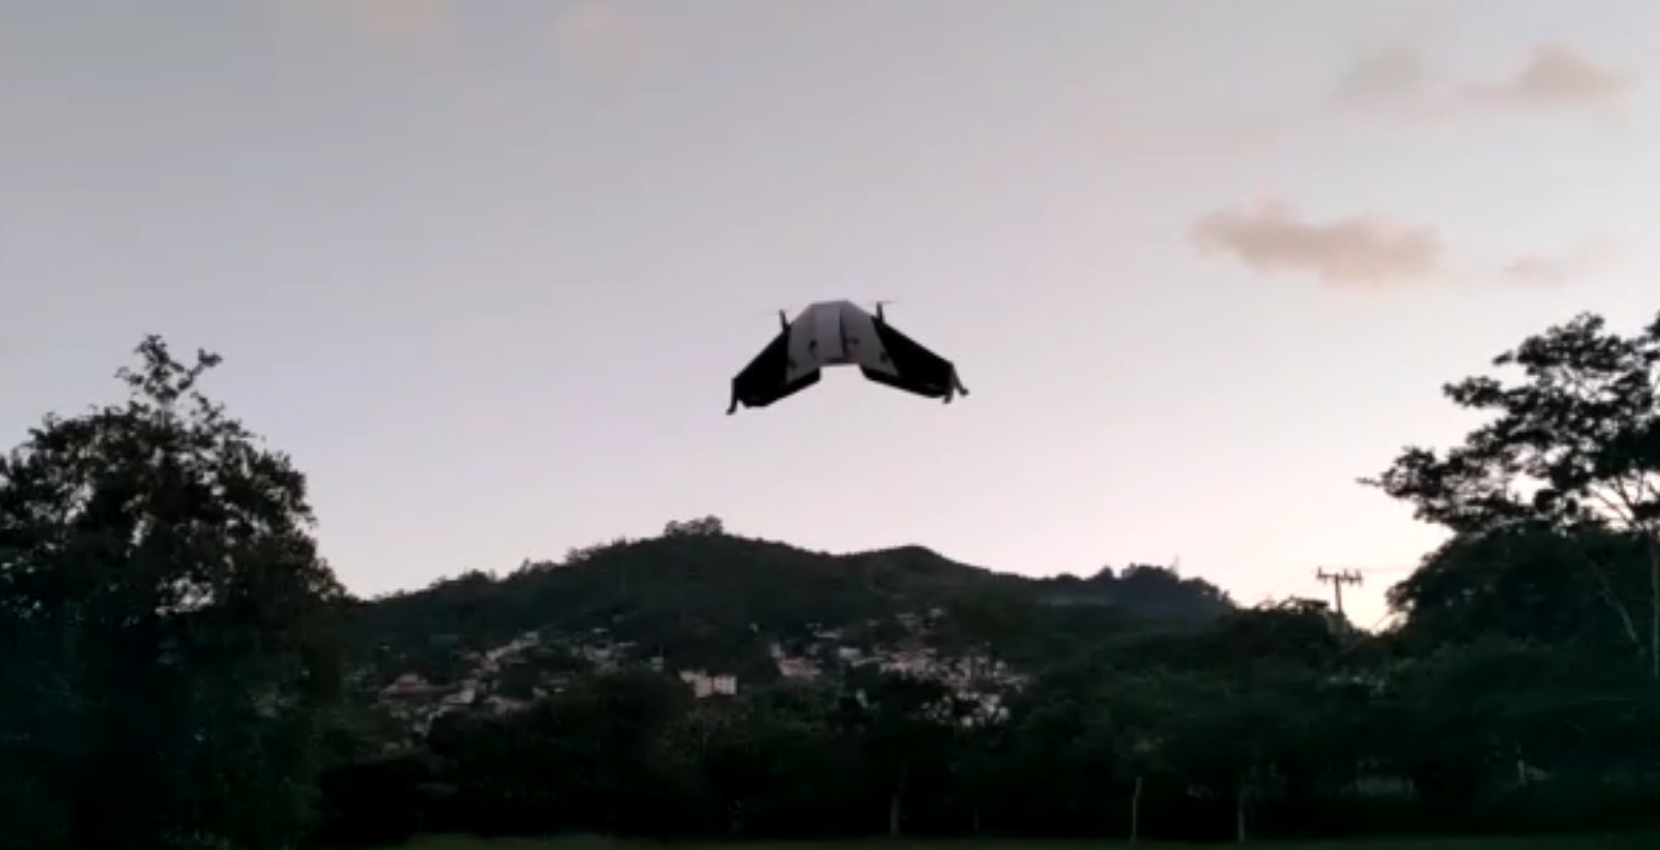
\includegraphics[width=0.7\linewidth]{figs/flight1-photo.png}
  \caption{Photo of first test flight.}
  \label{fig:flight1-photo}
\end{figure}
	






